\startchapter{Making Socio Technical Congruence Actionable}
\label{chap:actionable}

\section{Recommender System: Chat To Succeed}

A project is comprised of multiple integration builds. An 
integration build is usually scheduled at regular intervals to 
compile software components into a running program. 

Most software projects have infrastructure in place that automatically builds the software system on a regular basis. If there are errors in this build, or if automated regression tests fail, then we consider this as a failed build.  Research shows that communication structures can be used 
to predict the outcome of a build~\cite{wolf:tr2008}.  Certain patterns of 
communication among team members who contribute to the 
code can determine if a build fails or succeeds. We expand this idea by providing specific recommendations of 
who should chat together to ensure a successful build.

We believe that when a build fails, there is a possibility that members of the software team coordinated poorly between the time the current build broke, and the last known successful build. One possible reason for this lack of coordination is that the team members who worked on interrelated components failed to inform each other about their changes. This brings us to the discussion of socio-technical congruence.

%(R1) - A clarification of what a "failed" build is. What is failing? Compilation? Regression testing?

\subsection{Socio-technical Gaps}


Socio-technical congruence defines the match of technical 
and social dependencies among people, for example tasks 
(technical) and task related communication (social)~\cite{cataldo:cscw:2006}. It 
compares a technical network to a communication network 
and identifies gaps where a coordination need exists, but no 
communication fills the gap. Recent work addressing socio-technical congruence assumes that each gap has a negative 
influence on the project, but there is no substantial evidence 
to support this. Further research has indicated that projects 
can succeed despite the existence of socio-technical gaps~\cite{marczak:re:2008}.

\begin{figure}[t]
\centering
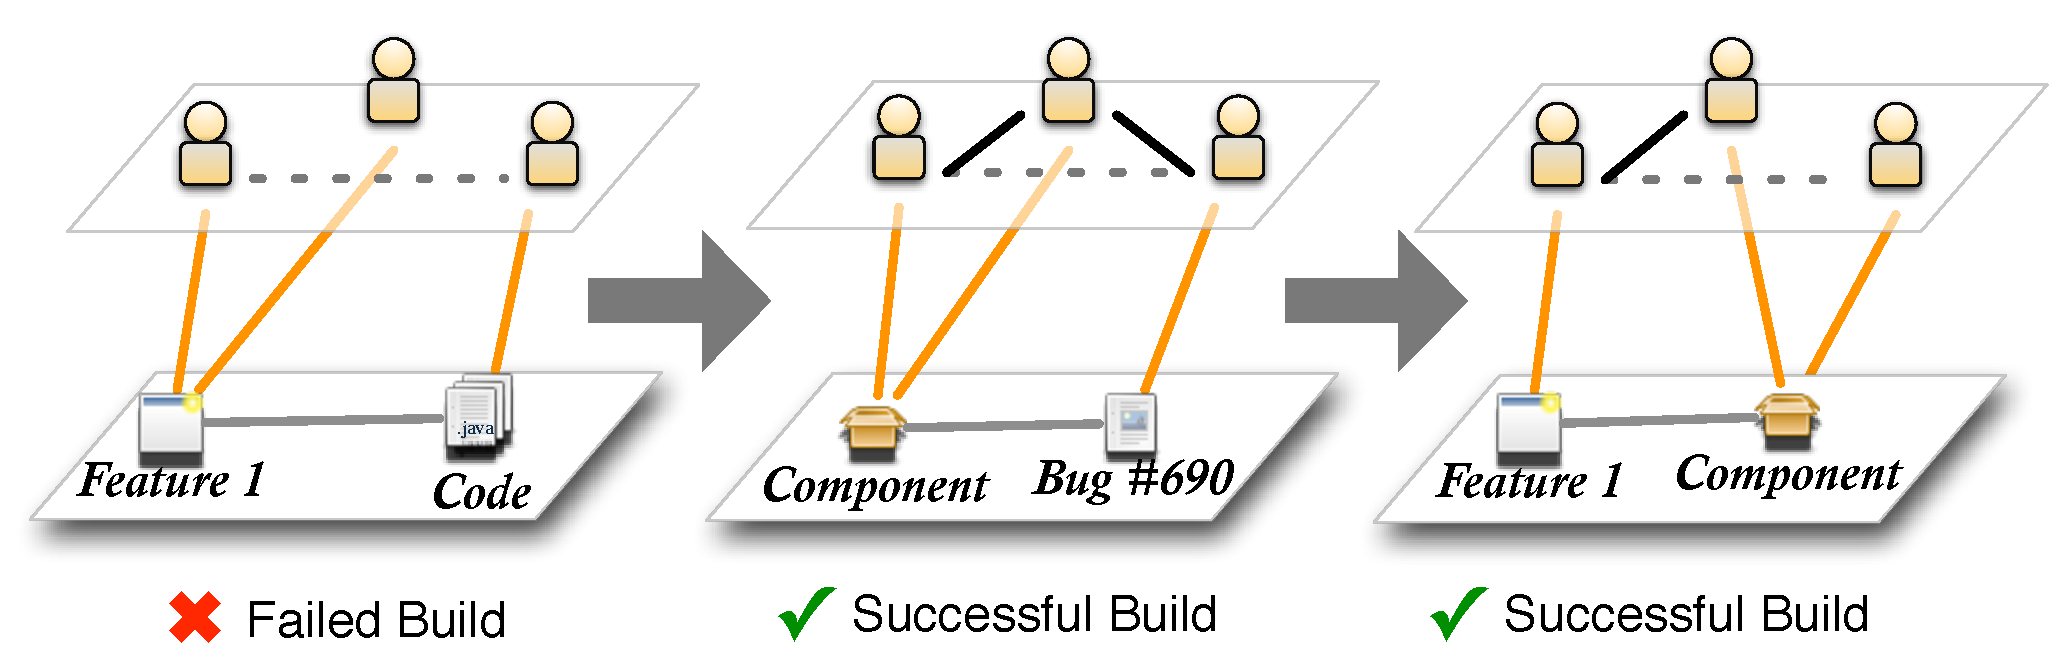
\includegraphics[width=0.9\columnwidth]{figures/bad-to-good}
\caption{Identifying failure inducing coordination gaps.}
\label{fig:multipleplanes}
\end{figure}

\subsection{Our Recommender System}
We propose a recommender system that recommends people you need to communicate with in order to prevent a 
failed build. The system will identify which gaps are bad 
and which are fine. A gap is bad if it is mainly present in 
failed builds whereas a gap is fine if it is present in both 
failed builds and successful builds. 
Figure~\ref{fig:multipleplanes} shows the social and technical networks for three 
builds. Developers are connected by working on the same 
artifact and by dependent artifacts. We see that the failed 
build exposes two socio-technical gaps. A first glance, this 
would lead to the conclusion that these gaps are bad. Further examination of the two following successful builds suggests that only one gap is bad since the other gap exists in 
one of the successful builds as well. 
To generate our recommendations we connect people in 
two ways: (1) on the technical level and (2) at the social 
level. 

\begin{description}
\item[Technical Level.] 
We mine repositories such as tracking systems and 
code for technical connections. For example, two developers have a technical connection if they work on 
dependent components or related bug fixes.
\item[Social Level.]
Social level connections can be found by mining email, chat, or comments~\cite{cataldo:cscw:2006}. In particular we need to 
focus on the tasks that are represented by the mined 
technical connections. 
\end{description}

We draw data from repository system by IBM called Jazz, which stores issue tracking, source code, and change sets in a single database. Jazz records associations between work items and change sets, as well as the results of integration builds. A build, therefore, includes the code contributions between the current integration build and the previous integration build. Thus, we can identify who has contributed to each integration build and who has coordinated about change sets that were included in a particular build.

We also draw data from open-source projects. In an open-source project that does not use Jazz, we can identify change sets from their source code repositories, and corresponding tracker items or development mailing list items based on commit logs. Prior to the data mining, the project's development system must be studied and understood in order to provide good recommendations.

%An open-source project may have multiple branches that are to be merged, such as a live stream for the current release, and a developer stream. We intend to treat each branch's change sets independently. For example, if only a subset of team members are permitted to check in change sets to a branch, then we know that coordination among that subset of team members only influences the outcome of integration builds on that branch. 

%(R2) 
%There is a critical area for improvement. The authors should emphasize the setup of the overall source control and build system when discussing their analysis approach for recommendations.  While the past congruence research focused on code changes and bug fixes - integration builds are much, much more than this.  How the different forks, versions, build scripts, unit tests, workspaces, and streams are connected together (and how all of this changes over time) strongly influence how integration builds operate.  This point was not clearly stated in the position statement.
% Hehe, we didn't use the word stream in our paper, but it seams that this reviewer is somewhat familiar with Jazz terminology

\subsection{Potential Challenges}
With this kind of study come a different number of challenges, in the following we list the four major challenges we think to encounter.
\begin{itemize}
\item \emph{Noise} can either be outliers in form of abnormal situations, such as a partly system failure that prevented recording the ongoing communication, or wrongly reported data.
First we plan to filter the data we use to see if the method would work, in a second step we need to evaluate the robustness to different levels and types of noise.
\item \emph{Incomplete data} goes along with the first challenge, since incomplete data can be seen as noise in form of wrongly recorded data as well.
We plan to deal with incomplete data similarly as we plan to deal with noisy data.
\item \emph{Correctness} of the recommendations is tricky to validate.
We plan to evaluate the recommendations via a case study, which observes a team and asking for feedback whether the recommendations would have helped. 
\item \emph{Usefulness} should be evaluated two fold. (1) We need to determine how early the recommendations become accurate enough and (2) we need to evaluate in a second case study if the recommendations lead to a better result with respect to a given measurement, such build success.
\end{itemize}
Besides those four challenges we of course need to deal with generalizability.
We aim to overcome this challenge by applying our approach to several major open source projects, such as Eclipse, Mozilla, and Apache, as well as closed software projects, depending on possible collaborations.

%(R1) - A brief discussion of the potential for noise and false positives in the data used to generate recommendations

%(R1) - Some proposed approaches to testing the recommendation algorithms, such as a Wizard of Oz approach to check the quality and relevance of the recommendations.

\section{A Course on Globally Distributed Software Development}
\section{Background and Related Work}
\section{Setting}
\section{Methodology}
\section{Findings}
\section{Discussion}
\section{Conclusions}
